\documentclass[conference]{IEEEtran}
\IEEEoverridecommandlockouts
% The preceding line is only needed to identify funding in the first footnote. If that is unneeded, please comment it out.
\usepackage{ctex}
\usepackage{cite}
\usepackage{amsmath,amssymb,amsfonts}
\usepackage{algorithmic}
\usepackage{graphicx}
\usepackage{textcomp}
\usepackage{xcolor}
\usepackage{listings}

\lstset{basicstyle=\small\fontencoding{T1}\ttfamily,breaklines=true}
\lstset{frame=shadowbox,tabsize=4}

\def\BibTeX{{\rm B\kern-.05em{\sc i\kern-.025em b}\kern-.08em
    T\kern-.1667em\lower.7ex\hbox{E}\kern-.125emX}}
\begin{document}

\title{Paxos 一致性协议及其实现
}

\author{\IEEEauthorblockN{1\textsuperscript{st} 王凯祺 \ 16337233}
\IEEEauthorblockA{\textit{数据科学与计算机学院} \\
wangkq3@mail2.sysu.edu.cn}
}

%\author{\IEEEauthorblockN{1\textsuperscript{st} Chongxuan Li}
%\IEEEauthorblockA{\textit{Dept. of Comp. Sci \& Tech.} \\
%Tsinghua University, Beijing, 100084, China \\
%licx14@mails.tsinghua.edu.cn}
%\and
%\IEEEauthorblockN{2\textsuperscript{nd} Kun Xu}
%\IEEEauthorblockA{\textit{TNList Lab} \\
%Tsinghua University, Beijing, 100084, China \\
%xu-k16@mails.tsinghua.edu.cn}
%\and
%\IEEEauthorblockN{3\textsuperscript{rd} Jun Zhu}
%\IEEEauthorblockA{\textit{State Key Lab of Intell. Tech. \& Sys.} \\
%Tsinghua University, Beijing, 100084, China \\
%dcszj@mail.tsinghua.edu.cn}
%\and
%\IEEEauthorblockN{4\textsuperscript{th} Bo Zhang}
%\IEEEauthorblockA{\textit{Center for Bio-Inspired Computing Research} \\
%Tsinghua University, Beijing, 100084, China \\
%dcszb@mail.tsinghua.edu.cn}
%}

\maketitle

\begin{abstract}
本文介绍 Paxos 一致性协议和它的实现。将一致性逻辑应用在网络设备上可以在数据中心中显著提高核心服务的性能。更重要的是,实现 Paxos 一致性协议还为数据层语言设计者提供了一种重要语法。在未来,我们终有一天能看到一致性协议能像现在的点对点通信协议一样,作为一个网络协议为大家服务。
\end{abstract}


\section{简介}

Paxos \cite{b13} 是一种解决\emph{一致性}问题(指在分布式计算中,让参与者在某些变量的值上达成一致的问题)而广泛使用的方法。Paxos 一致性协议可以用来构建容错系统,用以处理数据中心的核心业务,例如 OpenReplica \cite{b20} 、 Ceph \cite{b5} 和 Google's Chubby \cite{b4} 。由于大多数的数据中心应用程序高度依赖这些核心业务, Paxos 的性能会对数据中心的整体性能产生重要影响。

前人在工作中发现 \cite{b8} ,将 Paxos 逻辑应用在网络转发设备中能显著提高性能。特别地,将一致性应用到网络服务不仅能减少一致性信息传输所需的跳数,还能突破服务器上信息处理的瓶颈。前人还找到了一个充分的操作集合,使得能在交换机实现 Paxos 逻辑。但是到目前为止,在交换机上实现 Paxos 逻辑仍然非常困难,因为这需要硬件厂商的配合,需要自定义硬件实现。目前,网络计算硬件正在迅猛发展,有些硬件设备能提供自定义流水线处理数据包的接口,如 Barefoot networks \cite{b2} 生产的 PISA 芯片以及 Intel 的 FlexPipes \cite{b11} ,另外一些厂家如 Cisco 和 Cavium 在不久的将来也将生产类似的硬件设备。

本文将介绍 Paxos 的实现。尽管 Paxos 是一个相对简单的协议,在实现上它还是有不少细节的,因此涌现出许多关于 Paxos 实现的论文,力求简单\cite{b14}、可行\cite{b17}、可用\cite{b6}。本文与前人作品的不同之处在于,在网络转发设备上实现 Paxos 的过程中,我们发现了前人未提及过的新问题。

\section{Paxos 的背景}

状态机复制通常应用于复制服务,因此任意一台复制服务器上发生错误并不会影响正常复制服务器对客户端的服务。一致性协议规定了参与者如何传输和执行指令。状态机复制的实现就采用了一致性协议。

Paxos \cite{b13} 应该是使用得最广泛的一致性协议。参与者是若干相互交换信息的进程。参与者可以同时担任以下一种或多种角色:\emph{提议者}对分布式系统发出请求(提议一个值)、\emph{协作者}确定请求的次序、\emph{接受者}选择一个合适的值、\emph{学习者}对已经选择的值提供复制服务。

一个 Paxos 实例指的是用 Paxos 协议执行一次复制。当一个提议者发出请求时,就意味着实例的开始;当学习者知道接受者选择了哪个值时,意味着实例的终止。实例根据 Paxos 协议,依次处理每一轮。每一轮包含两个阶段,我们将在下文中给予解释。对于每一轮,一个担当提议者或接受者的进程在本轮中同时担当协作者。协作者是由应用程序特有的协议——协作者选举协议选举出。该协议不包含在 Paxos 协议中,因此不展开讨论。

\paragraph{阶段 1}
协作者选择一个唯一的轮序号 $rnd$ ,并要求接受者保证在任意实例中拒绝轮序号小于 $rnd$ 的任何请求(包括阶段 1 和阶段 2 的请求)。当多数接受者(记接受者的集合为 $Q_a$ )接受协作者的请求时,第一阶段结束。如果任意一个接受者已经在本实例中接受了一个值,接受者会将该值以及与该值对应的轮序号返回给协作者。

\begin{figure}
\centering
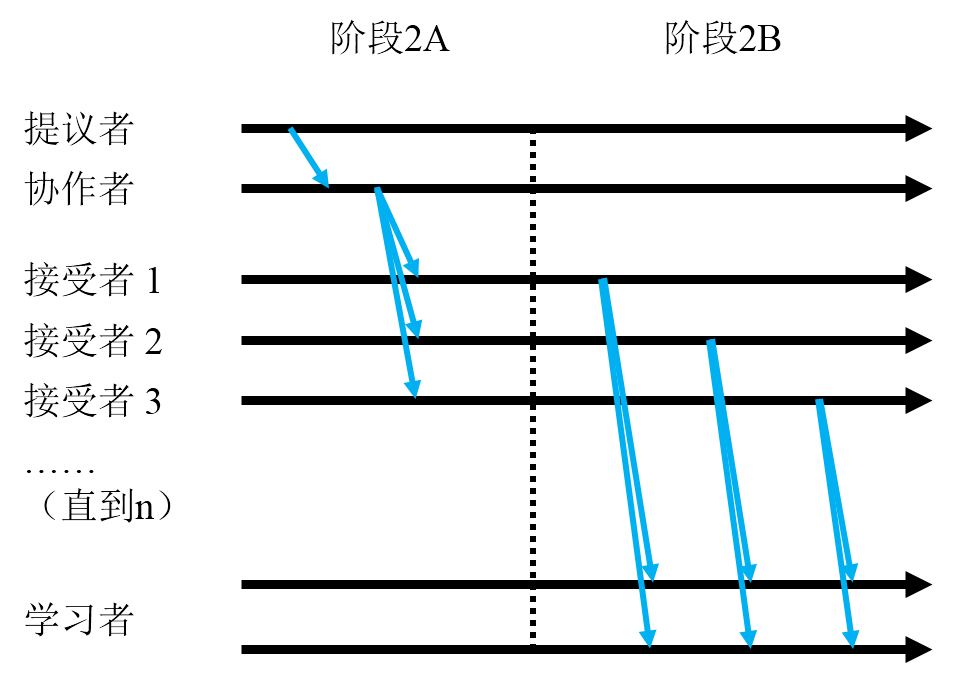
\includegraphics[scale=0.5]{img/image1.png}
\caption{Paxos 协议通信模式}
\label{l1}
\end{figure}

\paragraph{阶段 2}
图 \ref{l1} 解释了阶段 2 中 Paxos 参与者的通信模式。协作者按如下规则选择一个值:若在 $Q_a$ 中的所有接受者都没有接受过值,协作者可以选择任意值发送。若在阶段 1 中存在一个或多个接受者返回了值,那么在阶段 2 中协作者\emph{必须}选择最大轮序号 $vrnd$ 对应的值进行发送。在阶段 2 中,协作者在发送值的同时,也要发送轮序号(与阶段 1 一样)。接受者在接收到阶段 2 的请求后,如果该请求的轮序号不小于接受者在此前(包括阶段 1 和阶段 2)收到的轮序号的最大值,接受者将确认此消息;否则将拒绝确认。随后,接受者更新他们的 $rnd$ 以及 $vrnd$ 值。当多数接受者接受了相同的轮序号,一致性算法结束:该轮序号对应的值将被永久确定为该实例的值。这样,学习者可以通过监控接受者,或者从协作者接收决定信息来获得接受者的最终决定。

只要有一个正常(无故障)的协作者被选中,且存在多数(过半)正常的接受者,并且存在一个正常的提议者,那么每一个实例都会决出一个最终值。失效的协作者会被其他节点检测出来,其他节点将会选举出新的协作者。如果协作者没有接收到阶段 1 消息的回应,它可以重新发送(可能会用更大的轮序号)。当然这也适用于阶段 2 。

\section{基本表示}

为了在网络转发设备上实现 Paxos 协议,我们定义五个核心概念如下:

\begin{itemize}
\item \emph{头部字段}:一个数据包的头部包含的字段。开发者必须指明每个字段的长度。最多一个字段的长度为可变的。
\item \emph{分析器}:分析器描述了如何从数据包变换成语法分析后的表现形式。
\item \emph{映射表}:开发者必须定义一个从匹配字段到动作的映射表,即:若有一个数据包到达,网络转发设备上必须完成指定动作。
\item \emph{动作}:在映射表中被提及的动作。动作包含:修改字段、添加或删除头部信息、丢弃数据包或转发数据包、进行有状态的操作(如存储经过的数据包)等。
\item \emph{控制}:开发者必须指明映射表是如何构成的。
\end{itemize}

除了这五个基本概念以外,我们对 Paxos 的实现还需要使用\emph{寄存器}和\emph{元数据}。寄存器能以数组的形式记录一系列单元格的持久化状态。当声明一个寄存器时,开发者必须指定每个单元格的大小以及数组的大小。元数据跟寄存器的用法很类似,只不过它额外提供了存储易变的单数据包状态的机制。

\section{Paxos 的实现}

\begin{figure}
\centering

\includegraphics[scale=0.4]{img/image2.png}
\caption{以交换机为基础的 Paxos 层次架构。交换机硬件已用文字作区分。其它设备均为普通的服务器。每个学习者拥有 4 个网卡。}
\label{l2}
\end{figure}

图 \ref{l2} 解释了以交换机为基础的 Paxos 层次架构。交换机硬件已用文字作了区分。其它设备均为普通的服务器。跟传统的 Paxos 一样,我们有 4 种参与者角色:提议者、协作者、接受者和学习者。在以交换机为基础的 Paxos 中,\emph{协作者}和\emph{接受者}的功能用网络转发设备来实现。

在第 2 节中描述的 Paxos 协议是两阶段的,阶段 1 并不依赖于任何特定的值,故能提前预处理一个很大的边界值 \cite{b13}。预处理在以下两种情况需要重新计算:一是 Paxos 实例接近边界值,二是协作者变更(可能由失效导致)。因此,不失一般性地,我们在本文中只实现阶段 2 。我们的以交换机为基础的 Paxos 也遵循这个要求。

\subsection{Paxos 头部字段}

在 Paxos 协议中通信的所有数据包均为 UDP 数据包,均必须包含 Paxos 协议指定的头部字段。图 \ref{l3} 展示了头部字段和分析器的明确定义。头部信息包含以下 5 个字段:

\begin{itemize}
\item msgtype: 用以区分不同的 Paxos 信息(如阶段1A、阶段1B、阶段2A、阶段2B 等);
\item inst: 本条消息中包含的 Paxos 实例;
\item rnd: 本字段的含义取决于发送者的身份。若提议者发送消息,那么 $rnd$ 即为阶段 1 中的轮序号;若接受者发送消息,那么 $rnd$ 即为接受者为某提议投票的轮序号;
\item vrnd: 某个接受者投票的轮序号;
\item value: 提议的值,或者接受者为某提议投票的提议值。
\end{itemize}

\subsection{提议者}

我们把提议者的实现封装成一个库,并将 API 暴露给应用程序。API 仅包含一个方法 $submit$ ,用来给应用程序提交值并接收回应。提议者组件从应用程序中接收请求,创建 Paxos 信息后发送给协作者(阶段 2A 信息)。信息以多播的形式传输,这使得协作者和接受者能高效地广播消息到多个目标主机。

\subsection{协作者}

在 Paxos 中,协作者作为提议者们的代表,与接受者们协商请求。当提议者们同时提议一个值的时候,协作者就要将消息按一定顺序推送出去。当只有一个协作者的时候,即 Paxos 的原型,我们用一个单调递增的 inst 字段来为消息排序。

图 \ref{l4} 展示了协作者的实现逻辑。代码中执行了三个操作: (i) 复制下一个要用的实例号到消息头部; (ii) 将实例号自增; (iii) 存储新的实例号。我们使用 reg\_inst 寄存器将实例号保存起来。当协作者收到了一条合法的消息,它将把数据包传给 tbl\_sequence 表,由表匹配阶段 2A 的信息并执行 handle\_2a 操作。handle\_2a 执行以下操作:首先从寄存器中读取实例号,并将它写到 inst 头部字段;然后,将序列号自增并将新值写道寄存器;最后, tbl\_sequence 将控制权交回给 control 代码段,由 control 代码段将数据包转发给目标。

\begin{figure}
\centering
\begin{lstlisting}
header_type paxos_t {
	fields {
		msgtype : 8;
		inst : INST_SIZE;
		rnd : 8;
		vrnd : 8;
		value : VALUE_SIZE;
	}
}

parser parse_paxos {
	extract(paxos);
	return ingress;
}
\end{lstlisting}
\caption{Paxos 头部字段和分析器}
\label{l3}
\end{figure}

\begin{figure}
\centering
\begin{lstlisting}
register reg_inst {
	width : INST_SIZE;
	inst_count : 1;
}

action handle_2a() {
	register_read(paxos.inst, reg_inst, 0);
	add_to_field(paxos.inst, 1);
	register_write(reg_inst, 0, paxos.inst);
}

table tbl_sequence {
	reads { paxos.msgtype : exact; }
	actions { handle_2a; _nop; }
	size : 1;
}

control ingress {
	/* process other headers */
	if (valid(paxos)) {
		apply(tbl_sequence);
	}
}
\end{lstlisting}
\caption{协作者代码实现}
\label{l4}
\end{figure}

\subsection{接受者}

接受者从协作者中接收消息,然后决定接受还是拒绝这个提议。因此,接受者在整个系统里有保证整个系统一致性的作用。为了实现这个功能,接受者必须维护和访问之前他们通过的所有提议记录。这些状态并不会无限制地增长下去,它会周期性地删减。为了简化问题,我们并没有在代码中实现“删减”功能。

当接受者接收到一条消息时,它必须从存储器中读取本实例中最新的轮序号,与发来的数据包中的轮序号作比较。若这条消息拥有一个比之前每次都大的轮序号,接受者必须根据它的类型进行处理:(i) 若为阶段 1A 的消息,则用该数据包的值更新本地寄存器; (ii) 若为阶段 2A 的消息,则必须更新状态并转发该数据包。

\begin{figure}
\centering
\begin{lstlisting}
header_type paxos_metadata_t { fields { rnd : 8; } }
metadata paxos_metadata_t meta_paxos;
register rnds {	width : 8; inst_count : NUM_INST; }
register vrnds { width : 8; inst_count : NUM_INST; }
register values { width : VALUE_SIZE; inst_count : NUM_INST; }
action read_rnd() { register_read(meta_paxos.rnd, rnds, paxos.inst); }
action handle_1a() {
	modify_field(paxos.msgtype, PAXOS_1B);
	register_read(paxos.vrnd, vrnds, paxos.inst);
	register_read(paxos.value, values, paxos.inst);
	register_write(rnds, paxos.inst, paxos.rnd);
}
action handle_2a() {
	modify_field(paxos.msgtype, PAXOS_2B);
	register_write(rnds, paxos.inst, paxos.rnd);
	register_write(vrnds, paxos.inst, paxos.rnd);
	register_write(values, paxos.inst, paxos.value);
}
table tbl_rnd { actions { read_rnd; } }
table tbl_acceptor {
	reads { paxos.msgtype : exact; }
	actions { handle_1a; handle_2a; _drop; }
}
control ingress {
	/* process other headers */
	if (valid(paxos)) {
		apply(tbl_rnd);
		if (meta_paxos.rnd <= paxos.rnd) {
			apply(tbl_acceptor);
		} else {
			apply(tbl_drop);
		}
	}
}
\end{lstlisting}
\caption{接受者代码实现}
\label{l5}
\end{figure}

图 \ref{l5} 为接受者的代码实现。接受者需要维护多个有状态的结构体。我们使用了元数据 meta\_paxos 来存储接受者投票给哪一个轮序号,以及 3 个寄存器来存储 rnd, vrnd, value 。

程序的入口在 control 代码块。当一个数据包发来时,它将传递到两个表中。第一个表 tbl\_rnd 调用了 read\_rnd 操作来复制该实例中当前轮到元数据中;然后将存储器中的轮序号与当前轮序号作比较,若当前轮序号比存储器中的轮序号大,则这个数据包将被传送到接受者表 tbl\_acceptor 中;否则将被丢弃。

接受者表 tbl\_acceptor 引入了两个动作,分别对应两种不同的 Paxos 消息类型。handle\_1a 动作将消息类型设置为阶段 1B ,从存储器中读取 vrnd 和 value ,并把它们写到数据包中对应的字段中,然后更新轮寄存器。handle\_2a 动作根据数据包的头部字段更新 rnds, vrnds, values 寄存器,接受提议,并将消息类型设置为阶段 2B 。

\subsection{学习者}

学习者必须从接受者中接收投票,少数服从多数。每个学习者通过不同的网络接口与所有的接受者相连。学习者通过不同的网络接口可以分辨出数据包是由哪个接受者发出的。当收到一条阶段 2B 消息时,学习者要解析实例号、轮序号和值。学习者可以维护一个二维数组来存储这些信息,第一维用于存储实例,第二维表示接口。当作出决定后,学习者将执行请求,然后把反馈发给提议者。

\section{总结}

灵活的硬件以及数据层程序设计语言会给网络带来很深远的影响。在 Paxos 这个案例中,有了前二者的软硬件结合,可以显著提升数据中心的性能。在本论文中,我们阐述了如何实现 Paxos 。这个实现在数据层语言中迈出了第一步,也为之后一致性协议的设计奠定了基础。

\begin{thebibliography}{00}
\bibitem{b2} P. Bosshart, G. Gibb, H.-S. Kim, G. Varghese, N. McKeown, M. Izzard, F. Mujica, and M. Horowitz. ``Forwarding Metamorphosis: Fast Programmable Match-Action Processing in Hardware for SDN''. In SIGCOMM Conference on Applications, Technologies, Architectures, and Protocols for Computer Communication, pages 99-110, Aug. 2013.
\bibitem{b4} M. Burrows. ``The Chubby Lock Service for Loosely-Coupled Distributed Systems''. In USENIX Symposium on Operating Systems Design and Implementation, pages 335-350, Nov. 2006. 
\bibitem{b5} Ceph. http://ceph.com
\bibitem{b6} T. D. Chandra, R. Griesemer, and J. Redstone. ``Paxos Made Live: An Engineering Perspective''. In ACM Symposium on Principles of Distributed Computing, pages 398-407, Aug. 2007. 
\bibitem{b8} H. T. Dang, D. Sciascia, M. Canini,, F. Pedone, and R. Soule. ``NetPaxos: Consensus at network speed''. In 1st ACM SIGCOMM Symposium on Software Defined Networking Research, pages 59-73, June 2015. 
\bibitem{b11} L. Jose, L. Yan, G. Varghese, and N. McKeown. ``Compiling packet programs to reconfigurable switches''. In USENIX Symposium on Networked Systems Design and Implementation, pages 103-115, May 2015. 
\bibitem{b13} L. Lamport. ``The Part-Time Parliament''. ACM Transactions on Computer Systems, 16(2), 133-169, May 1998.
\bibitem{b14} L. Lamport. ``Paxos made simple''. ACM SIGACT News, 32(4), 18-25, Dec. 2001. 
\bibitem{b17} D. Mazieres. ``Paxos made practical''. Unpublished manuscript, 2007. 
\bibitem{b20} OpenReplica. http://openreplica.org
\end{thebibliography}

\end{document}
